\section{Using existing libraries and APIs}
\label{sec:apivisions}

In the next sections we will show you how to deal with multimedia contents from scratch, with special attention to image classification using state-of-the-art libraries. However, it might be a good idea to begin by using some existing libraries that directly implements multimedia analysis or by connecting to commercial services to deploy classification tasks remotely using their APIs. There is a vast variety of available libraries and APIs, which we cannot cover in this book, but we will briefly mention some of them that may be useful in the computational analysis of communication.

One example in the field of visual analytics is the \textit{optical character recognition} (OCR). It is true that you can train your own models to deploy multi-class classification and predict every letter, number or symbol in an image, but it will be a task that will take you a lot of effort. Instead, there are specialized libraries in both R and Python such as \pkg{tesseract} that deploy this task in seconds with high accuracy. It is still possible that you will have apply some pre-processing to the input images in order to put them on shape. This means that you may need to use packages such as \pkg{PIL} or \pkg{Magick} to improve the quality of the image by cropping it or by reducing the background noise.  In the case of PDFs files you will have to convert them first into images and then apply OCR.

In the case of more complex audio and image documents you can use more sophisticated services provided by private companies (i.e. Google, Amazon, Microsoft, etc.). These commercial services have already deployed their own machine learning models with very good results. Some times you can even customize some of their models, but as a rule their internal features and configuration are not transparent to the user. Moreover, these services offer friendly APIs and normally a free quota to deploy your first exercises.

To work with audio files, many social researchers might need to convert long conversations, radio programs, or interviews to plain text. For this propose, \textit{Google Cloud} offer the service \textit{Speech-to-Text}\footnote{https://cloud.google.com/speech-to-text}  that remotely transcribe the audio to a text format supporting multiple languages (more than 125!). With this service you can remotely use the advanced deep learning models created by Google Platform from your own local computer (you must have an account and connect with the proper packages such as \pkg{googleLanguageR} or \pkg{google-cloud-language} in Python).

If you apply either OCR to images or Speech-to-Text recognition to audio contents you will have juicy plain text to conduct NLP, sentiment analysis, topic modelling, among other techniques.  Thus, it is very likely that you will have to combine different libraries and services to perform a complete computational pipeline, even jumping from R to Python, and vice versa!

Finally, we would like to mention the existence of commercial services of \textit{autotaggers}, such as Google's Cloud Vision, Microsoft's Computer Vision or Amazon's Recognition. For example, if you connect to the services of Amazon's Recognition you can not only detect and classify images, but also conduct sentiment analysis over faces or predict sensitive contents within the images. As in the case of Google Could, you will have to obtain commercially sold credentials to be able to connect to Amazon's Recognition API (also with a free initial quota). This approach has two main advantages. The first is the access to a very well trained and validated model (continuously re-trained) over millions of images and with the participation of thousands of coders. The second is the scalability because you can store and analyse images at scale at a very good speed using cloud computing services.

\begin{figure}
\centering
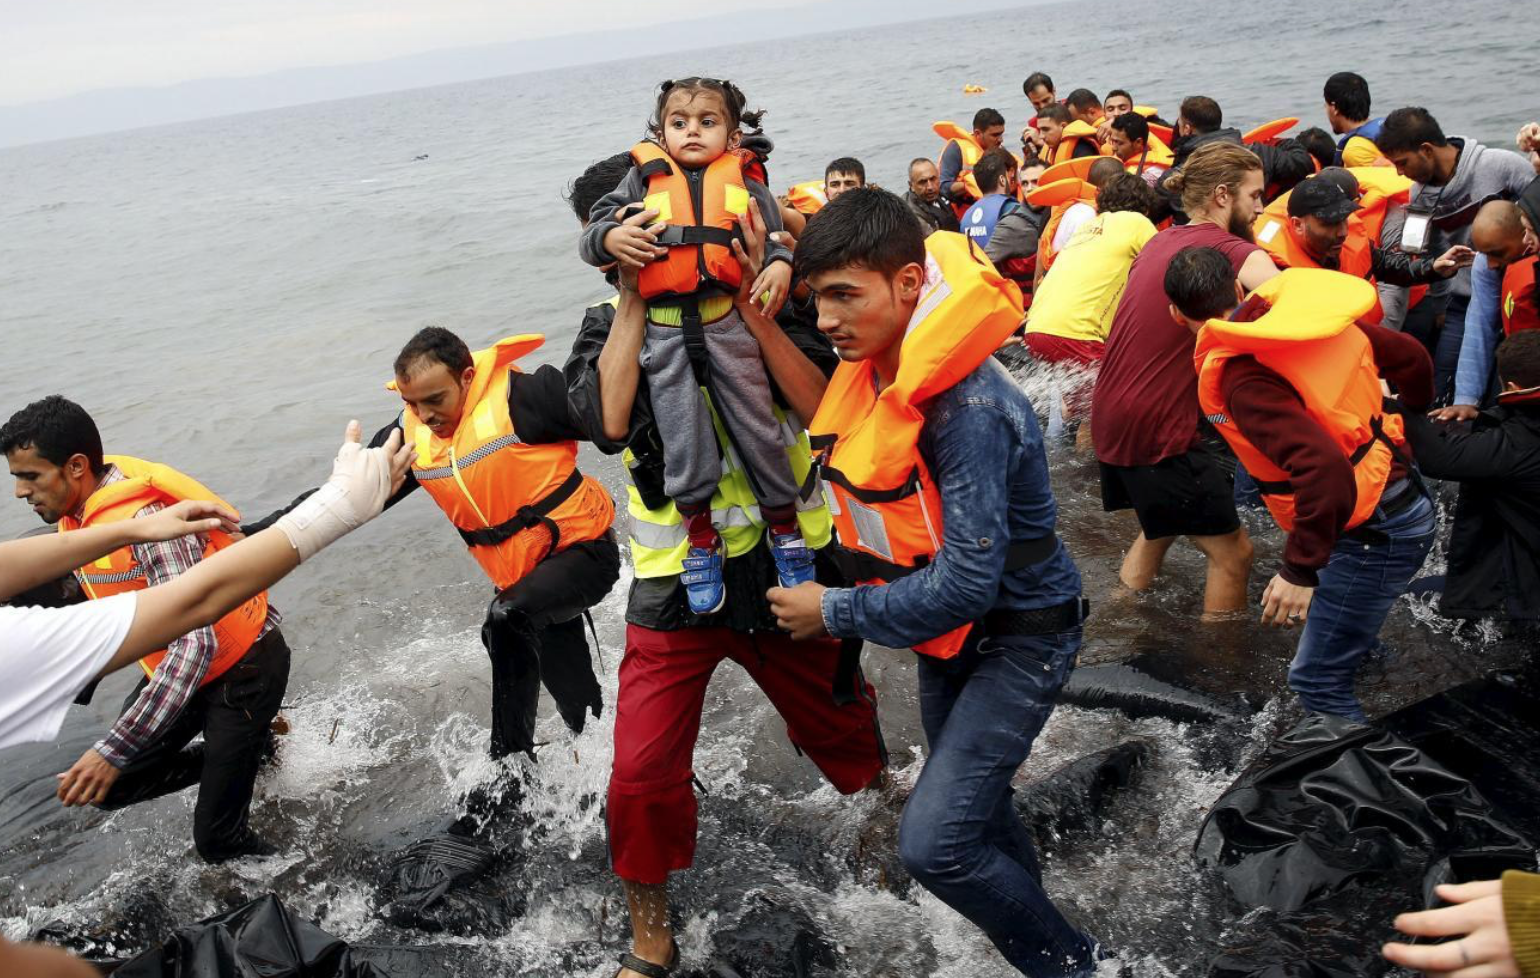
\includegraphics[width=0.9\linewidth]{figures/ch15_refugees.png}
\caption{By using Amazon's Recognition API
A photograph of refugees on a lifeboat, used as an input for Amazon's Recognition API. The commercial service detects in the pictures classes such as clothing\, apparel\, human\, person\, life jacket or vest.}
\label{fig:refugees}
\end{figure}

As an example, you can use Amazon's Recognition to detect objects in a news photograph of refugees in a lifeboat (Figure~\ref{fig:refugees}) and you will obtain a set of accurate labels: \textit{Clothing} (99.95\%), \textit{Apparel} (99.95\%), \textit{Human} (99.70\%), \textit{Person} (99.70\%), \textit{Life jacket} (99.43\%) and \textit{Vest} (99.43\%). With a lower confidence you will also find labels such as \textit{Coat} (67.39\%) and \textit{People} (66.78\%). This example also highlights the need for validation, and the difficulty of grasping complex concepts in automated analyses: While all of these labels are arguably correct, it is safe to say that they fail to actually grasp the essence of the picture and the social context. One may even go as far as saying that -- knowing the picture is about refugees -- some of these labels, were they given by a human to describe the picture, would sound pretty cynical.

In Section~\ref{sec:cnn} we will use this very same image (stored as \texttt{my\_image2\_RGB}) to detect objects using a classification model trained with an open-access database of images (ImageNet). You will find that there are some different predictions in both methods, but especially that the time to conduct the classification is shorter in the commercial service, since we don't have to train or choose a model. As you may imagine, you cannot neither modify the commercial models nor have access to their internal details, which is a strong limitation if you want to build your own and customized classification system.
